\section{Dataset and Evaluation Metric}
\label{sec:data}

We provide a textual QA dataset with aspects, an evaluation metric and two baselines for this spect-based QA pairs generation task. We will introduce the dataset and the evaluation metric in this section.

\subsection{Dataset}
SQuAD2.0 is a well known QA textual dataset with the amount of annotated QA pairs from documents.
Therefore in this paper, we just add the aspect keywords for each paragraph of the SQuAD2.0 dataset to support our experiments.

\paragraph{Dataset Creation}
To allocate a suitable aspect keyword for each paragraph in SQuAD, we convert the paragraphs to original Wikipedia pages and extract the closest heading as the aspects.
In this step, to ensure that the paragraphs in SQuAD are consistent with the corresponding paragraphs in the original Wikipedia, 
we did not select wiki dumps as the source to obtain aspect keywords but crawled the most similar wiki texts which are distributed between 2012 and 2016.

However, SQuAD only annotated a part of paragraphs from Wikipedia and there is a lack of ground truth QA of the unannotated paragraphs.
To make a suitable evaluation of our frameworks, we merge the paragraphs with annotated QA pairs as the input document $D$.
%Finally, we construct the dataset with the format $<$document, aspect keyword, paragraph, QA pairs$>$.

Figure \ref{fig:wiki} shows an example of a Wikipedia page with the information followed by the aspect-based QA dataset.

\begin{figure*}[th]
    \begin{center}
    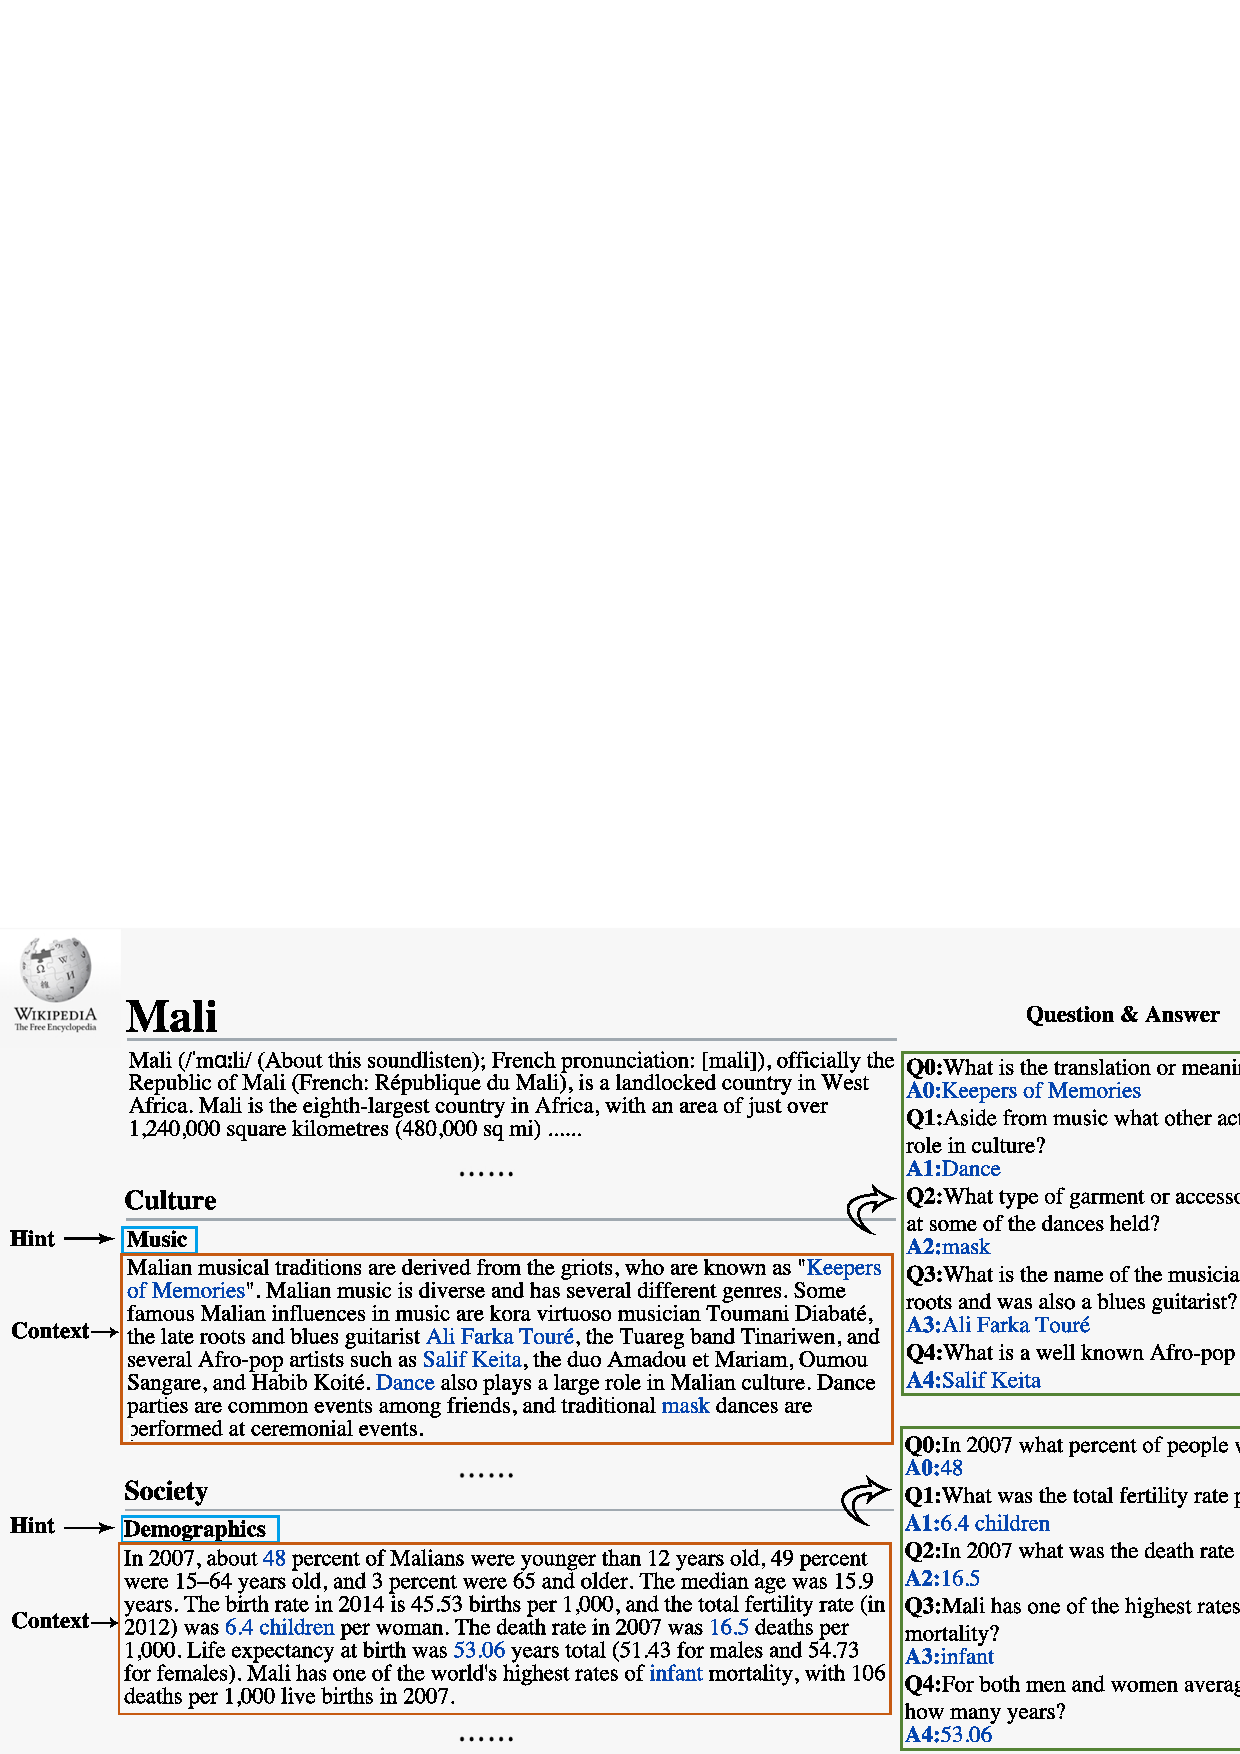
\includegraphics[width=0.8\textwidth]{pic/Wikipedia.pdf}
        \caption{\label{fig:wiki} An example of Wikipedia page \textbf{Black Death} and the information followed by our aspect-based QA dataset.
        The blocked context is the paragraph included in SQuAD2.0. The aspect keyword is the closest heading of the paragraph and the QA pairs on the right side are annotated in SQuAD2.0. The emoji in this figure is to show the relevance between the QA pairs and  aspect.}
    \end{center}
\end{figure*}

\paragraph{Annotated Evaluation Set}
Although the paragraph is highly relevant to its aspect, not all of the QA pairs in SQuAD are related to this aspect.
The example in Figure \ref{fig:wiki} also shows this phenomenon. 
This paragraph talks about the causes of black death, in which QA1 and QA2 are relevant to this aspect.
However, QA0 is irrelevant which is talking about the details far from the topic.

We randomly select 100 QA pairs to judge whether they are relevant to their aspects, and find there are 60.58\% relevant samples.
Due to the noise in our dataset, there are two master students asked to label the relevance between the hint and the QA pair.

We assume that noisy samples are still aspect useful.
To ensure sufficient training samples, we only manually select the relevant test data to do the evaluation.
%The labeled intersect positive samples are formed as the evaluation dataset.

\paragraph{Size of the dataset}
Following the same data split method as Zhao et.al.~\shortcite{zhao2018paragraph},  we regard the dev* set as the test set, and split train set into train and dev sets randomly with the ratio of 9:1.
After adding the aspect words to each paragraph and manually labeling the QA pairs relevant to the corresponding aspects as the evaluation set, the size of our dataset is shown in Table \ref{tab:size}:
\begin{table}[th]
\scriptsize
\centering
\begin{tabular}{ccccc}
\toprule[1.5pt]
 & \textbf{\#Docs} & \textbf{\#Paragraphs} & \textbf{\#Aspects} & \textbf{\#QA pairs} \\ 
\midrule[1pt]
\textbf{train} & 398 & 17188 & 6421 & 78723 \\ 
\textbf{dev} & 44 & 1847 & 777 & 8098 \\ 
\textbf{annotation test} & 11 & 285 & 20 & 1018 \\ 
\bottomrule[1.5pt]
\end{tabular}
\caption{\label{tab:size} Size of our aspect-based dataset.}
\end{table}

\subsection{Evaluation Metric}
\label{sec:metric}
For individual modules, we use the well-known metrics to evaluate the performance of each model.
For paragraph retrieval, we choose the average F1@$K$ and MRR@$K$ to score the list of paragraphs ranked with the relevance to the aspect, where $K$ is the number of the ground truth paragraphs.
For answer span extraction, we evaluate the performance of answer spans as Subramanian et al.~\shortcite{subramanian2017neural} did. 
We calculate the token-level F1 score matrix of elements $f_{i,j}$ between the two answers $a_i$ and $a_j$ and obtain the mean precision, recall, F1 among the paragraphs.
For question generation, we choose the widely used generation metrics, such as BLEU, METEOR, and ROUGE-L which are implemented by Sarma's work~\cite{sharma2017relevance}.

For the entirety of QA pairs, we design an end-to-end metric to score each pair of generated QA.
We use the aspect as a unit to judge the QA pairs.
Given a document and an aspect keyword, there is a set of ground truth QA pairs $(Q, A)$ and a set of generated QA pairs $(\hat{Q}, \hat{A})$.
We calculate the QA score matrix $M$ of elements $S_{i,j}$ between the ground truth QA pair $(q_i, a_i)$ and $a_j$ and predicted QA pair $(\hat{a_j}, \hat{q_j})$.
The pairwise score is:
\begin{equation}
\scriptsize
\begin{aligned}
\text{J-BLEU} &= Jaccard(a_i, \hat{a_j})\times \text{BLUE}(q_i, \hat{q_j})\\
\text{J-METEOR} &=Jaccard(a_i, \hat{a_j})\times \text{METEOR}(q_i, \hat{q_j})\\
\text{J-ROUGE} &= Jaccard(a_i, \hat{a_j})\times \text{ROUGE}(q_i, \hat{q_j})\\
\end{aligned}
\end{equation}

Where $a_i$ and $\hat{a_j}$ are the tokens of ground truth answer span and predicted answer span respectively, and $q_i$ and $\hat{q_j}$ are the strings of ground truth question and predicted question respectively.

Max-pooling along the ground truth axis of score matrix $M$ assesses the precision of each QA pair generated for the aspect: $p_j=max_i(S_{i,j})$.
Max-pooling along the predict axis of $M$ assesses the recall:  $r_i=max_j(S_{i,j})$.
The multi-QA metric is:
\begin{equation}
\scriptsize
\begin{split}
&Precision=mean(p)\\
&Recall=mean(r)\\
&F1=\frac{2\times Precison\times Recall}{Precison+Recall}
\end{split}
\end{equation}


